% SPAR Midterm Report Template
% Compatible with arXiv (TeX Live 2023+, pdflatex)
%
% To compile: latexmk -pdf report.tex
% Or use the build scripts: build report.tex

% ============================================================================
% DOCUMENT CLASS
% ============================================================================
% Options: midterm | final | arxiv
% - midterm: For mid-program report
% - final: For end-of-program report
% - arxiv: For converting your report into a preprint for arXiv
\documentclass[midterm]{sparreport}

% ============================================================================
% METADATA
% ============================================================================
\title{Your Report Title Here}

\author{
  \textbf{Your Name}\\
  \texttt{your.email@example.com}
  % Optional: Add institution/affiliation (recommended for arXiv mode):
  % \\
  % Your Institution
  % Add more authors (including mentors) with \and:
  % \and
  % \textbf{Mentor Name}\\
  % \texttt{mentor@example.org}\\
  % Mentor Institution
}

\sparround{Fall 2025}

% ============================================================================
% DOCUMENT BEGINS
% ============================================================================
\begin{document}

\maketitle

% ============================================================================
% ABSTRACT (100-200 words)
% ============================================================================
% Provide an overview of your research question and why it matters for
% addressing risks from advanced AI. Describe your methodological approach
% and any preliminary findings. If working on technical safety or security,
% mention the specific threat model, vector, or vulnerability. Keep this
% accessible to readers outside your subfield. No footnotes or citations.
\begin{abstract}
Your abstract goes here. Describe your research question, why it matters for AI safety, your approach, and preliminary findings (100-200 words).
\end{abstract}

% Keywords (optional but recommended, especially for arXiv submission)
\keywords{alignment research \and machine learning \and AI safety}

% ============================================================================
% INTRODUCTION (100-350 words)
% ============================================================================
% Describe the specific problem or question you're investigating and explain
% why it matters. Make clear what gap in existing work you're trying to fill
% or what risk you're addressing. Situate your project relative to existing
% approaches or prior work. Articulate what success would look like for your
% project—what would you need to demonstrate or discover for this research
% to be valuable?
\section{Introduction}

Introduce your research problem and explain its significance for AI safety. Describe the gap you're filling or risk you're addressing. Explain what success would look like for this project.

% ============================================================================
% METHODOLOGY (200-500 words)
% ============================================================================
% Describe your research approach clearly enough that someone could understand
% what you're doing and roughly replicate it. For empirical work, include your
% experimental setup, systems or datasets, and evaluation metrics. For
% theoretical work, outline your framework, key assumptions, and approach to
% arguments or proofs. For policy research, describe your research design,
% data sources, and analytical approach.
\section{Methodology}

Describe your research approach and methods.

% Example subsections (optional):
% \subsection{Experimental Setup}
% \subsection{Dataset and Evaluation}
% \subsection{Analysis Framework}

% Example figure
% \begin{figure}[htbp]
%   \centering
%   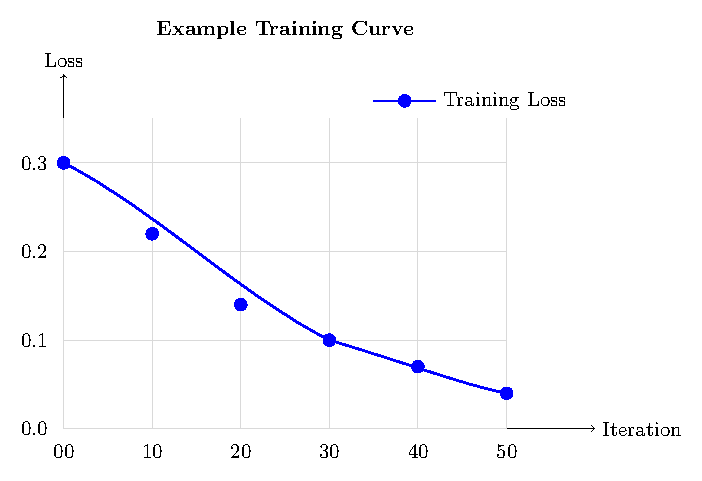
\includegraphics[width=0.7\textwidth]{figures/example-figure.pdf}
%   \caption{Example figure caption.}
%   \label{fig:example}
% \end{figure}

% Example table
% \begin{table}[htbp]
%   \centering
%   \caption{Example table caption.}
%   \label{tab:example}
%   \begin{tabular}{lcc}
%     \toprule
%     Method & Accuracy & Time \\
%     \midrule
%     Approach A & 85\% & 2.3s \\
%     Approach B & 92\% & 4.1s \\
%     \bottomrule
%   \end{tabular}
% \end{table}

% ============================================================================
% PRELIMINARY RESULTS (200-500 words)
% ============================================================================
% Present what you've found so far. For empirical work, focus on quantitative
% findings with visualizations. For theoretical work, focus on key insights or
% partial results. For policy research, present initial findings from your
% analysis. Use subheadings if helpful. It's normal for midterm results to be
% incomplete.
\section{Preliminary Results}

Present your findings so far. Use subsections and visualizations as appropriate.

% ============================================================================
% CHALLENGES & OPEN QUESTIONS (100-300 words, optional but encouraged)
% ============================================================================
% Be honest about obstacles you've encountered: technical difficulties, resource
% constraints, or conceptual challenges. Note any areas where you're still
% figuring things out or where the path forward is uncertain.
\section{Challenges \& Open Questions}

Describe obstacles you've encountered and areas of uncertainty.

% ============================================================================
% NEXT STEPS (150-400 words)
% ============================================================================
% Highlight what you will focus on and what you will try to accomplish during
% the next half of the program. What will you prioritize? What might you
% deprioritize or cut if needed?
\section{Next Steps}

Describe your planned next steps for the remainder of the program. What will you prioritize?

% ============================================================================
% WORKS CITED / BIBLIOGRAPHY
% ============================================================================
% The reference page lists all sources used for your project, including those
% cited in the review and methods sections. Ensure the citation style is
% consistent throughout.
%
% For arXiv submission: You MUST include the generated .bbl file!
% Compile with: latexmk -pdf report.tex (or pdflatex -> bibtex -> pdflatex -> pdflatex)
% Then submit both .tex and .bbl files to arXiv.

\bibliographystyle{plain}
\bibliography{references}

\end{document}
